\section{Plant}
\label{Chapter:Plant}
\subsection{Plant Description}
\begin{figure}[hbt]
    \centering
    \includegraphics{figures/ADIP_plant.png}
    \caption{ADIP in Up-Up configuration}
    \label{fig:ADIP}
\end{figure}
Dr Y. Nishi originally designed the ADIP for training purposes at Kawasaki Heavy Industry in Japan. Here, the pendulum is the top link and is driven by the rotating arm, which is the bottom link. A DC motor actuates the arm. It is, therefore, a single input multi output system where the angles of the arm, $\phi_1$, and the pendulum, $\phi_2$, are the outputs measured by incremental rotary encoders. It is worth noting that the dynamics of the ADIP are highly non-linear and chaotic. Additionally, the ADIP is an under-actuated system. This makes it a challenging problem for control. The ADIP has infinitely many fixed points, and of those, an important fixed point is the stable equilibrium of the system described as the `down-down' configuration, where both the arm and pendulum are in the downward position i.\,e. $\phi_1 = \phi_2 = \pi$ radians. This system is characterized by only one stable equilibrium point, and the rest of the fixed points constitute unstable equilibria. For the scope of this work, a set of unstable equilibria is described as the `up-up' configuration where both the arm and pendulum are positioned as $-\pi/2<\phi_i<\pi/2, i = 1,2$. The case of an up-up configuration when $\phi_1 = \phi_2 = 0$ is shown in Fig. \ref{fig:ADIP}.\\
% The software Quarc acts as an interface between Simulink and the actual plant to implement the synthesized controller. The Simulink model is converted into a C++ code and executed in a real-time environment by this software. A universal power
% module (UPM2410-PWM) converts the low-voltage signal from the PC into a current signal for the motor.
\newpage
\subsection{First-Principles Model}
\label{Sec:firstprinci}
\begin{figure}[H]
	\centering
	    \scalebox{.5}{\input{figures/externalize/FBD_ADIP.tex}}
		\caption{A schematic of the ADIP}
		\label{fig:ADIP_model}
\end{figure}
Consider a schematic ADIP shown in Fig. \ref{fig:ADIP_model} . The arm is of length $L_1$ and has a mass $m_1$ which is assumed to be concentrated at a distance $l_1$, the approximate centre of mass of the arm. Similarly, the pendulum is of length $L_2$ and has a mass $m_2$ assumed to be concentrated $l_2$, the approximate centre of mass of the pendulum. An encoder is placed at the link between the arm and the pendulum to measure the angle made by the pendulum with the vertical. The encoder, along with its mounting on the arm, has a mass $m_3$ located at $L_1$.\par
The states and inputs are defined in a right hand Cartesian coordinate system. Since the ADIP is a planar setup, only the $x$ and $y$ axes are considered. The angular rotation of the arm $\phi_1$, and of the pendulum $\phi_2$, are measured to the $y$ axis where a clockwise direction is positive. $\phi_1 = \phi_2 = \pi$ when the ADIP is in the stable equilibrium position.\par
The DC motor applies a torque $u_1$ to the arm, and the link between the arm and the pendulum is not actuated but free to rotate. As a consequence of the torque in the arm, a disturbance torque $u_2$ is experienced by the pendulum.
A few assumptions are made before deriving the dynamics of the system. These assumptions are referenced from those made for a similar system, the Furuta pendulum, as presented by Cazzolato et al., \cite{Cazzolato}. These are:
\begin{enumerate}
    \item The motor shaft and the arm are assumed to be rigidly coupled and infinitely stiff,
    \item The pendulum is assumed to be infinitely stiff,
    \item Only viscous friction at the joints with damping coefficients $C_{arm}$ and $C_{pend}$ for arm and pendulum respectively are considered. All other forms of damping, if necessary, can be added to the final governing equations of motion appropriately.  
\end{enumerate}
The equations of motion for the ADIP are formulated through the Euler-Lagrangian energy-based method. This formulation needs only the change in the kinetic and potential energies of the system.\par
Since the arm and the pendulum are rigid bodies and have uniformly distributed mass along their length, it is convenient to calculate the total change in kinetic energy, $T$, as the sum of kinetic energies of the masses $m_1$, $m_2$ and $m_3$. \\
\begin{equation*}
    T = \frac{1}{2}J_{arm}\Dot{\phi_1}^2 + \frac{1}{2}J_{pend}\Dot{\phi_2}^2 + \frac{1}{2}m_2{v_{c}}^2 + \frac{1}{2}J_{enc}\Dot{\phi_1}^2  + \frac{1}{2}J_{motor}\Dot{\phi_1}^2 \;,
\end{equation*}
where $J_{arm}$ is the moment of inertia of the arm at the point of rotation of the arm, $J_{pend}$ is the moment of inertia of the pendulum about its centre of mass, $v_c$ is the velocity of the centre of mass of the pendulum, $J_{enc}$ is the moment of inertia of mass $m_3$  at the point of rotation of the arm, and  $J_{motor}$ is the rotational inertia of the DC motor. The rotational kinetic energy caused due to the rotational inertia of the DC motor is also added to the total kinetic energy since this value is not negligible and has a considerable effect on the dynamics of the system. \par
The change in potential energy of the system is similarly calculated as:
\begin{align*}
    V &= V_{1} + V_{2} + V_{3}\;, \\
    V &= m_1gl_1(1-\cos{\phi_1}) + m_2g(L_1(1-\cos{\phi_1}) + l_2(1-\cos{\phi_2})) + m_3gL_1(1-\cos{\phi_1})\;.
\end{align*}
\par
The equations of motion for the ADIP can then be computed from Eqs. \ref{eq:LagrangeEqn} and \ref{eq:lagdyn} as
\begin{equation}
\label{eq:ADIP_dyn}
    \mathbf{M}\mathbf{\Ddot{q}} + \mathbf{C(q,\Dot{q})}\mathbf{\Dot{q}} + \mathbf{G(q)} = \mathbf{u}\;,
\end{equation}
where
\begin{align*}
\mathbf{M} &=    \begin{bmatrix}
        \theta_1  & \theta_3c_{12}\\
        \theta_3c_{12} & \theta_2  
\end{bmatrix}\; , \quad
\mathbf{C} = \begin{bmatrix}
C_{arm} & \theta_3\Dot{\phi_2}s_{12}\\
-\theta_3\Dot{\phi_1}s_{12} & C_{pend}
\end{bmatrix}\;,\\
\mathbf{G} &=    \begin{bmatrix}
        -\theta_4g\sin(\phi_1)\\
        -\theta_5g\sin(\phi_2) 
\end{bmatrix}\;, \\
\textup{with}\\
\theta_1 &= J_{arm} + J_{motor} + J_{enc} + m_1l_1^2 + m_2L_1^2 \;,\\
\theta_2 &= m_2l_2^2 + J_{pend} \;,\\
\theta_3 &= m_2L_1l_2 \;,  \\
\theta_4 & = m_1l_1 + m_2L_1 + m_3L_1 \;, \\
\theta_5 &= m_2l_2 \;,\\
s_{12} &= \sin(\phi_1 - \phi_2) \quad \textup{and} \quad c_{12} = \cos(\phi_1 - \phi_2). 
\end{align*}
For the ADIP, $\mathbf{q} = [\phi_1 ~~ \phi_2]^{\top}$, $\mathbf{u} = [u_1 ~~ 0]^{\top}$.
% and $D = \frac{1}{2}C_{arm}\Dot{\phi_1}^2 + \frac{1}{2}C_{pend}\Dot{\phi_2}^2$.
The physical parameters of the ADIP and their values are listed in Table \ref{tab:params}. The masses and the geometrical entities were measured physically when the plant was disassembled. The motor parameters were taken from the motor manual, which can also be found in the appendix of this report. The friction is considered to be viscous and is estimated through the system identification tool-box in Matlab by comparing the simulated and experimental data.
\newpage
\begin{table}[H]
    \centering
    \begin{tabular}{lll}
         \toprule
         Parameter   & Description                              & Value\\
         \midrule
         $L_1$       & Length of arm                            & $0.154~m$\\
         $L_2$       & Length of pendulum                       & $0.186~m$ \\
         $l_1$       & Distance to C.G of the arm               & $0.077~m$\\
         $l_2$       & Distance to C.G of the pendulum          & $0.093~m$\\
         $m_1$       & Mass of arm                              & $0.13~kg$\\
         $m_2$       & Mass of pendulum                         & $0.07~kg$\\
         $m_3$       & Mass of encoder assembly                 & $0.04~kg$\\
         $J_{arm}$   & Moment of Inertia of arm                 & $3.00 \times 10^{-4}~kg{\cdot}m^2$\\
         $J_{pend}$  & Moment of Inertia of pendulum            & $2.02 \times 10^{-4} ~ kg{\cdot}m^2$\\
         $J_{motor}$ & Moment of Inertia of motor               & $1.58 \times 10^{-4}~kg{\cdot}m^2$\\
         $J_{enc}$   & Moment of Inertia of encoder assembly    & $7.37 \times 10^{-4}~kg{\cdot}m^2$\\
         $C_{arm}$   & Viscous damping co-efficient of arm      & $2.89 \times 10^{-3}~N{\cdot}s/m$\\
         $C_{pend}$  & Viscous damping co-efficient of pendulum & $1.41 \times 10^{-5}~N{\cdot}s/m$\\
         $g$         & Acceleration due to gravity              & $9.81~m/s^2$\\
        \bottomrule
    \end{tabular}
    \caption{ADIP parameters}
    \label{tab:params}
\end{table}

\subsection{Data-Driven Model}
\label{Chapter:Data}
A data-driven model is derived solely from available measurement data with almost no assumptions made about the plant. However, one can always augment the obtained measurements by \textit{lifting} the measurements through some linear or nonlinear functions of the same. This enables one to predict the behaviour of a model over longer time spans and deduce a linear operator which governs the evolution of these measurements. This linear operator is obtained by applying the previously mentioned methods like DMD, EDMD or SINDy. This section elaborates on the observables that are relevant for this thesis work. As previously discussed in Chapter \ref{Chapter:Prelims}, the choice of observables is crucial to estimate the Koopman operator, but discovering the `correct' observables is still an ongoing topic of research. Currently, there are several approaches to approximate the observables, for example, exploiting apriori knowledge of system dynamics \cite{Brunton_K_invariant_sub}, physical intuition of the system dynamics \cite{Cisneros.2020}, applying popular function approximators like radial basis functions \cite{Korda_edmd_conv} or polynomial basis and Fourier basis functions \cite{Abraham}, estimating the dominant candidates in a dynamic equation through sparse regression as done in SINDy \cite{SINDy} etc. \par 
During the course of this thesis work, all of the above-stated options were explored. While some worked well for prediction, the same could not be applied for control purposes. The reason why this could not be done is left to further research. However, it was observed that SINDy worked well in predicting the dynamics of the system, and this could be used as a first step in identifying reliable observables, at least for prediction, if not control. It was also observed that the measured state of the system predicted the dynamics of the system very well in the vicinity of the equilibrium and as the system moved farther away, the addition of some nonlinear states helped in better prediction of the system states. This is better explained in the Chapter~\ref{Chapter:Sim} where the effect of the choice of observables is evaluated in open-loop and closed-loop system identification.
\par 
In this thesis, a combination of states and nonlinear functions form the observables vector. Again, the choice of observables vary with the purpose. Many different combinations of observables were tried and for the purpose of the Chapter~\ref{Chapter:Sim}, four different vectors of observables are defined as follows
\begin{equation}
    \label{eq: obs1}
\mathbf{\Psi}_1 = [\phi_1 \quad \phi_2 \quad \dot{\phi}_1\quad \dot{\phi}_2 \quad u]^\top \in \mathbb{R}^5 \;,
\end{equation}
Thus, $\mathbf{\Psi}_1$ is just the state variables $\boldsymbol{\phi}^\top$ augmented with the input variable. \par
The state variables is augmented by a vector of polynomials up to second degree of the states which form the second observable vector,
\begin{align}
    \mathbf{\Psi}_2 &= [\boldsymbol{\phi}^\top \quad \psi_1\quad \psi_2 \quad \dots \quad \psi_{10} \quad u]  \in \mathbb{R}^{15}\;,\\
    \psi_i &= \phi_1^{\alpha_i}\phi_2^{\beta_i}\dot{\phi}_1^{\gamma_i}\dot{\phi}_2^{\delta_i} \;,
\end{align}
where $\alpha_i,\beta_i,\gamma_i,\delta_i$ are non-negative numbers and index $i$ tabulates all the combinations such that $\alpha_i+\beta_i+\gamma_i+\delta_i \leq Q$ and $Q>1$ defines the largest allowed polynomial degree. In the above case, $Q = 2.$\par
The third observables vector extends $\mathbf{\Psi}_2$ by including a combination of polynomial and sine functions of the state variables,
\begin{equation}
    \mathbf{\Psi}_3 = [\boldsymbol{\phi}^\top \quad \boldsymbol{\psi}^\top \quad \phi_1s_1 \quad \phi_1s_2 \quad \phi_1c_1 \quad \phi_1c_2 \quad \phi_2s_1 \quad \dots \quad \dot{\phi_2}c_2 \quad u] \in \mathbb{R}^{31}\;,
\end{equation}
where $s_1 = \sin{\phi_1}$, $c_1 = \cos{\phi_1}$ and similarly for others. Note that only the first two states were considered for the sine and cosine functions. Including the derivatives did not improve the prediction significantly and hence were discarded.\par
Finally, a combination of state variables and radial basis functions was also used. A \textit{radial function} is a real-valued function $\kappa$, that is radially symmetric around some point called the function's centre. This can be either the origin so that, $\kappa(\mathbf{x}) = \kappa(\norm{\mathbf{x}})$, or in general, some other point $\mathbf{c}$ so that $\kappa(\mathbf{x,c}) = \kappa(r)$, where $ r = \norm{\mathbf{x-c}}_2$ is the Euclidean distance between the points $\mathbf{x}$ and $\mathbf{c}$. Radial functions are typically used as a basis (and hence the name) to construct an approximation $\tilde{f}$, of a function of the form $y_i = f(\mathbf{x}_i)$ such that,
\begin{equation}
    \tilde{f}(\mathbf{x}) = \sum_{i=1}^N \boldsymbol{w}_i \kappa(\norm{\mathbf{x}-\mathbf{c}_i}) \;,
\end{equation}
where the approximating function $\tilde{f}$ is represented as a sum of $N$ radial basis functions~(RBFs), each associated with a different centre $\mathbf{c}_i$, and weighted by an approximate coefficient $\boldsymbol{w}_i$. The weights $\boldsymbol{w}_i$ are determined by ensuring that the approximation will exactly match the given data at data points i.e., $\tilde{f}(\mathbf{x}_i) = y_i $. This is accomplished by using the matrix methods of linear least squares, as the approximating function is linear in the weights $\boldsymbol{w}_i$. A detailed treatment of RBFs can be found in \cite{RBF}. There are several different types of radial basis functions, for example, gaussian RBFs, multi quadratic RBFs, polyharmonic RBFs, thin-plate splines etc. Thin plate spline RBFs usually work very well for function approximations \cite{Korda_edmd_conv} and are independent of any manual tuning parameters except for the choice of function centres. In this thesis work, therefore, 50 thin-plate spline RBFs are used along with the state vector to form the fourth observable vector,
\begin{align}
    \mathbf{\Psi}_4 &= [\boldsymbol{\phi}^\top \quad \kappa_1 \quad \kappa_2 \quad \dots \quad \kappa_{50} \quad u] \in \mathbb{R}^{55}\;,\\
    \textup{where} \notag \\
    \kappa(\boldsymbol{\phi}) &= \norm{\boldsymbol{\phi} - c}_2^2\log{(\norm{\boldsymbol{\phi} - c}_2)} \;.
\end{align}
In this thesis, the centres are chosen randomly within a set defined by the operating range of the system. Figure \ref{fig: RBF_centres} shows a selection of such centres and Figure \ref{fig: thinplate} shows a graph of the thin plate  spline RBF centred at the origin ($c = 0$). It is clearly seen that the value of $\kappa$ increases with the distance of the function from the centre. Therefore, it can be interpreted as if the RBF will be inactive when the centres are chosen near or at the measured data points, which is what is required since the observables vector also contains the measured state as observables. 
% 
\begin{figure}[ht]
\centering
\begin{subfigure}[t]{1\textwidth}
    \centering
    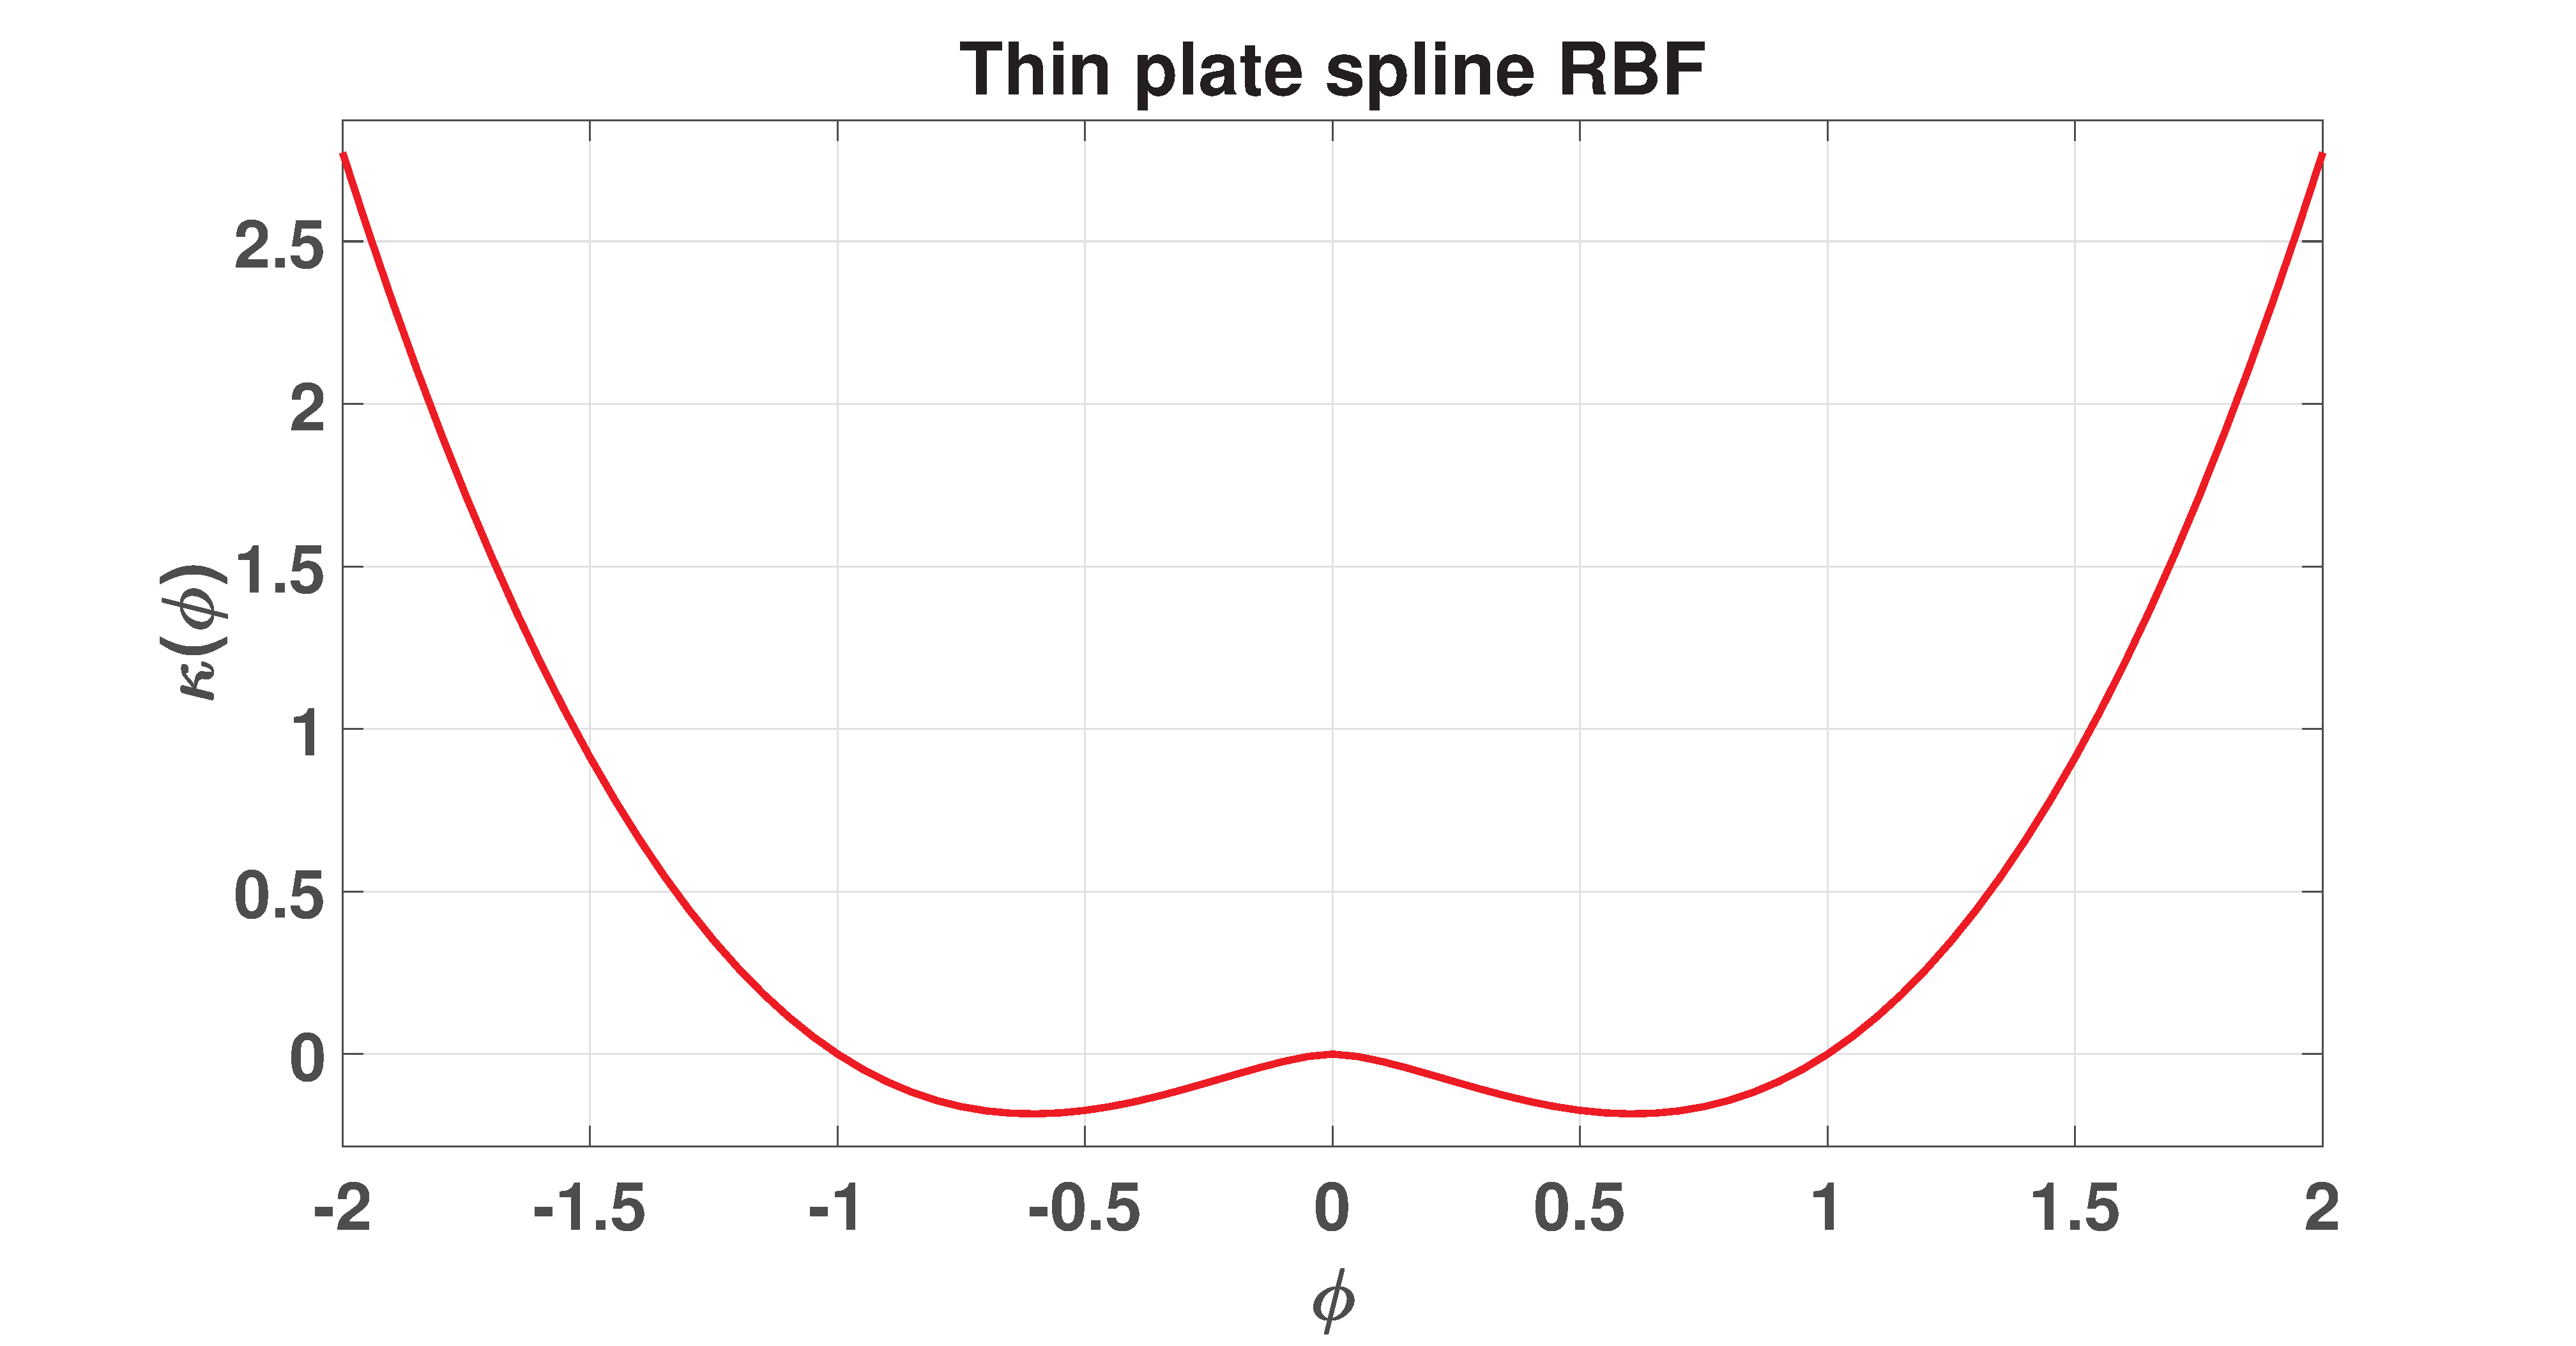
\includegraphics[width=0.75\linewidth]{figures/thinplate}
    \caption{Thin plate spline RBF}
    \label{fig: RBF_centres}
\end{subfigure}
\begin{subfigure}[t]{0.75\textwidth}
    \centering
    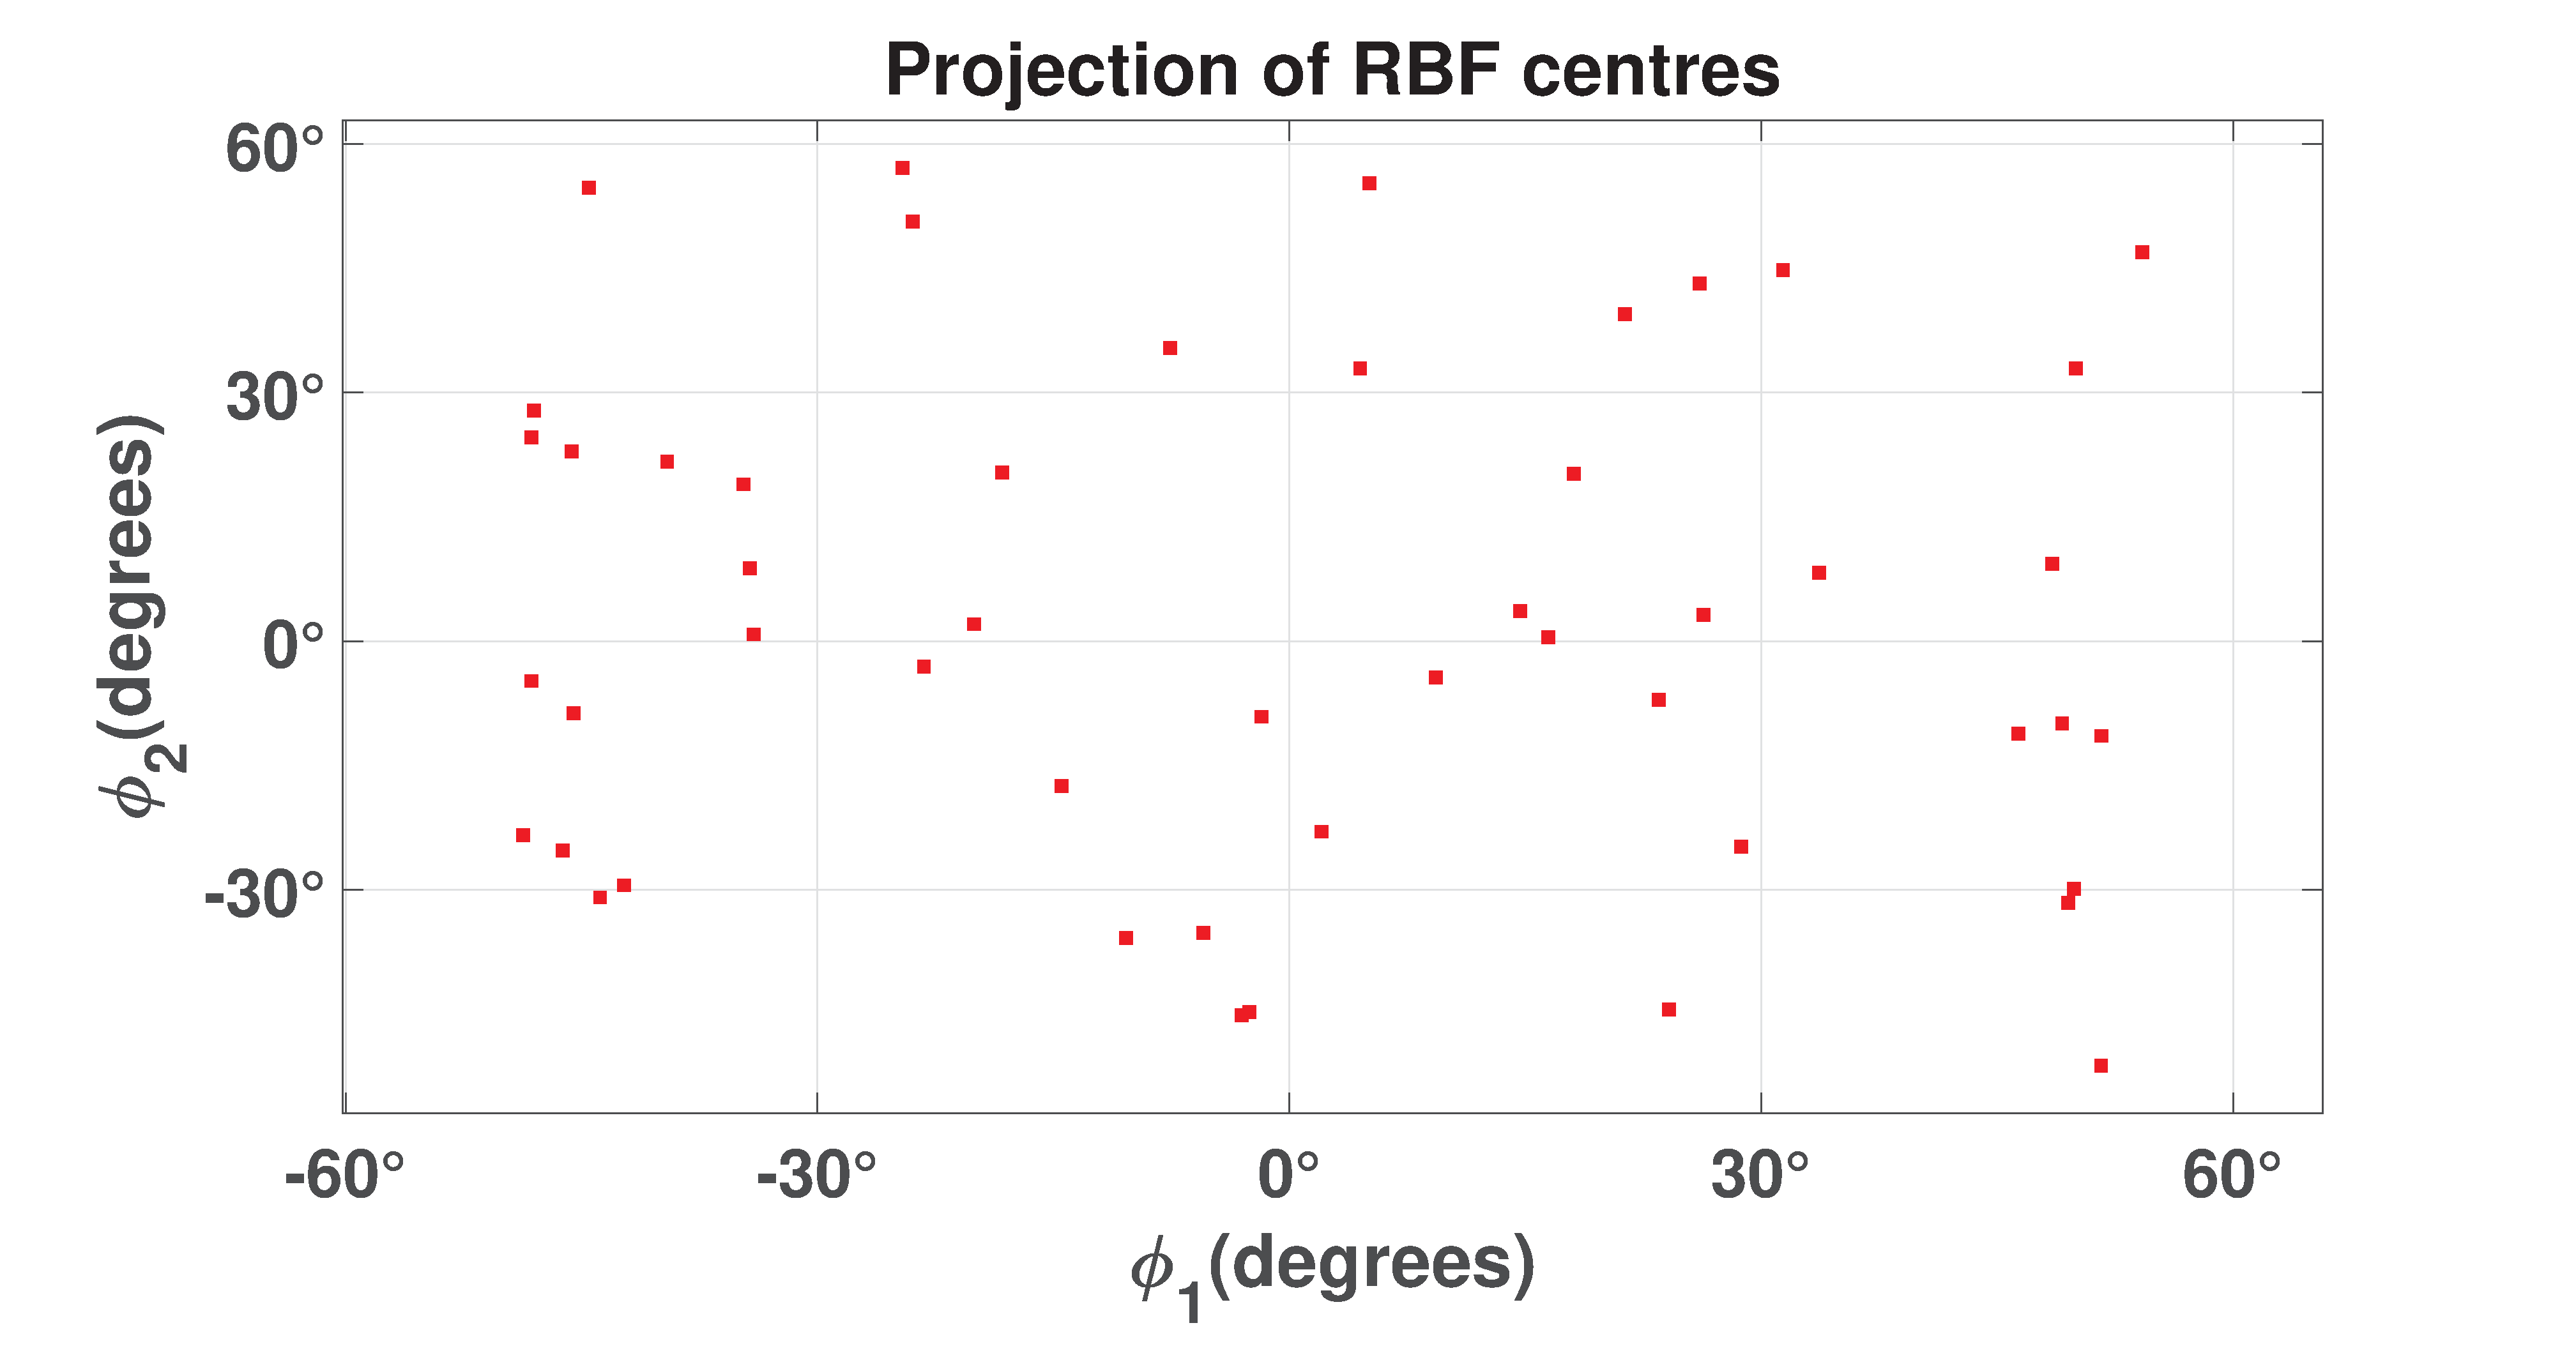
\includegraphics[width=1\linewidth]{figures/RBF_centres}
    \caption{RBF centres projected onto a plane for $\mathbf{\Psi_4}$ }
    \label{fig: thinplate}
\end{subfigure}
\caption{Thin plate splines RBF and the centres}
\end{figure}


